
% "Станет проще"

\documentclass[a4paper,12pt]{article} % тип документа
\usepackage{cmap}
% report, book

%  Русский язык

\usepackage[T2B]{fontenc}			% кодировка
\usepackage[utf8]{inputenc}			% кодировка исходного текста
\usepackage{graphicx}
\usepackage[english,russian]{babel}	% локализация и переносы


%отступ
\usepackage[left=2cm,right=2cm,
    top=2cm,bottom=2cm,bindingoffset=0cm]{geometry}

% Математика
\usepackage{amsmath,amsfonts,amssymb,amsthm,mathtools}
\usepackage{csvsimple}
\usepackage{multirow}
\usepackage{wasysym}
\usepackage{subcaption}
\usepackage{verbatim}
%\usepackage{ae,aecompl} better q
\usepackage{float}
\usepackage{enumerate}
\usepackage[dvipsnames]{xcolor}
\usepackage{rotating}
\usepackage[hidelinks]{hyperref} % Hide links

%Заговолок
%\graphicspath{ {images/} }


\begin{titlepage}
\author{Соловьянов Михаил}
\title{Вопросы к работе по напылению диода Шоттки}
\date{\today}
\end{titlepage}



\begin{document} % начало документа
\maketitle


\section{Вопросы по физике}
\begin{itemize}
  \item Что такое диод?
  \item Какие у диода бывают параметры (хар-ки)?
  \item Что такое полупроводник?
  \item Что такое легирование?
  \item Что такое полупроводник P и N типа?
  \item Какие леганты вы можете назвать?
  \item Какую точную гидродинамическую аналогию диода вы можете назвать?
  \item Чем диод шоттки отличается от обычного диода?
  \item Что такое зоны?
  \item Какие параметры металла и полупроводника определяют какие качества диода Шоттки?
  \item Что такое омический контакт?
  \item Как суметь предугадать проявление диода или омического контакта в соответсвующей структуре металл полупроводник?
  \item ***\footnote{Для особо интересовавшихся} Как устроен светодиод?
\end{itemize}

\section{Вопросы по процессам}

\begin{itemize}
  \item Что такое маска в процессе производства полупроводников?
  \item Зачем нам нужна была маска?
  \item В какой установке проводилось напыление? Как она устроена?
  \item Зачем напылять в вакууме?
  \item ** \footnote{Для тех кто в теме} Что такое резист?
  \item Что такое Имплантация?
\end{itemize}

\section{Вопросы по электронике}

\begin{itemize}
  \item Что такое прямое напряжение диода?
  \item Что такое обратное напряжеие диода?
  \item Что в документации обозначено как прямой ток диода?
  \item Какие применения диоду вы можете назвать?
  \item Когда диод шоттки применять лучше обычного диода?
  \item Зачем светодиоду резистор?
  \item Обьясните как работает диодный мост?
\end{itemize}

\section{Задачи}
  \subsection{Задача про выпрямительный диод}
Я пытаюсь подобрать выпрямительные диоды для диодного моста для зарядки для телефона. Она будет преобразовывать переменный ток из розетки (230В 50Гц), в USB (5В 2А), какие характеристики диода мне нужно взять во внимание при разработке такой зарядки? Принять минимальный КПД самого устройства 70\%. Выпрямительный мост это конструкция из четырех диодов собранных ромбиком (см. Рис.), которая превращает синус, или любые переменные токи, отражая ту их часть которая находится снизу наверх. Предложите конкретную модель подходящего светодиода.
\begin{figure}[H]
\centering
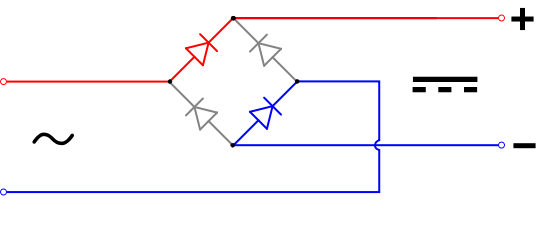
\includegraphics[width=0.7\textwidth]{bridge.png}
\caption{Диодный мост}
\end{figure}





  \subsection{Distortion}
  Покажите как будет выглядеть выходное напряжение на таком фильтре? Как вы думаете, как оно будет звучать по сравнению с изначальным?
  \begin{figure}[H]
  \centering
  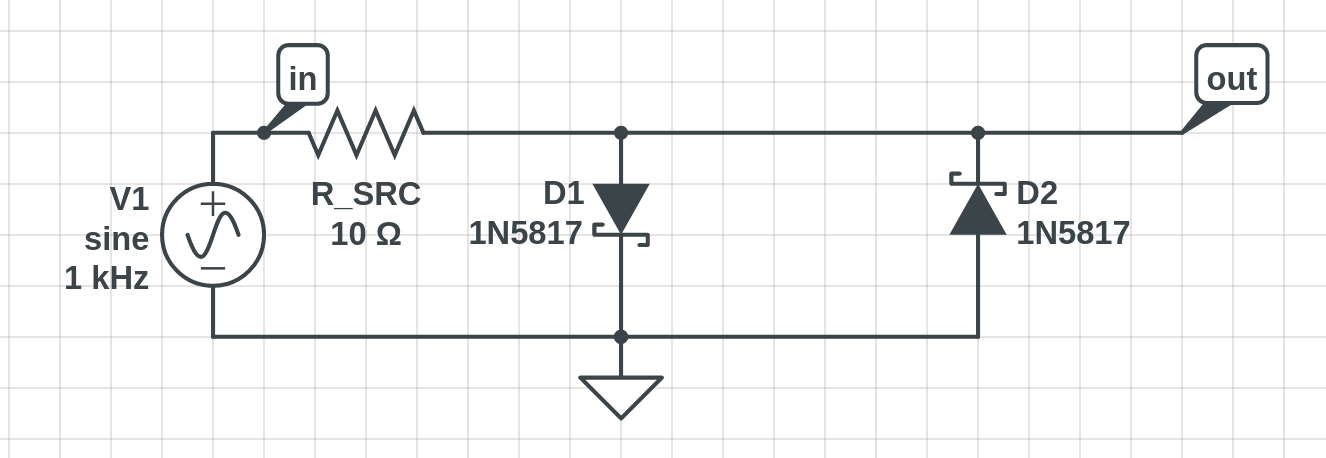
\includegraphics[width=0.7\textwidth]{task1.png}
  \caption{Схема фильтра}
  \end{figure}


  \subsection{Светодиоды}

  \subsubsection{Один светодиод}
  Рассчитайте резистор для последовательного включения с таким светодиодом: \url{https://www.nteinc.com/specs/3000to3099/pdf/nte3019.pdf} Напряжение питания 10В.

  \begin{figure}[H]
  \centering
  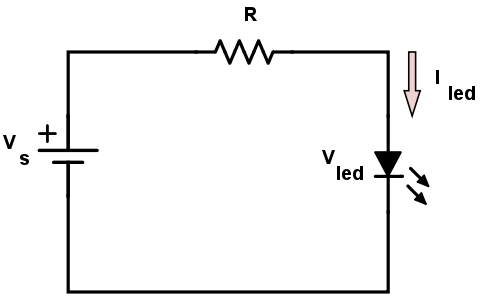
\includegraphics[width=0.4\textwidth]{external.png}
  \caption{Схема Включения одного диода}
  \end{figure}

  \subsubsection{Лента}
  Имеется лента из 5 светодиодов (вот такой даташит \url{https://www.nteinc.com/specs/3000to3099/pdf/nte3019.pdf}). Как рассчитать необходимое последовательное сопротивление для питания от 12В, чтобы она не сгорела?

  \subsection{Емкость обедненной области}\\
  **** WARNING:  DECEPTIVELY DIFFICULT CONCEPT ****\\

  Попытайтесь найти обьем обедненной области при приложении к ней напряжения. Известно легирование полупроводников (концентрация носителей) и прочие данные. Постройте график $C(V)$\\
  \textit{ \url{https://ecee.colorado.edu/~bart/book/book/chapter4/ch4_3.htm}}\\
  \textit{ \url{https://inst.eecs.berkeley.edu/~ee105/fa00/lectures/Lectw4.PDF}}

  % https://inst.eecs.berkeley.edu/~ee105/fa00/lectures/Lectw4.PDF


  %\subsection{Неправильное питание}

\end{document}
